% TODO: vymyslet lepší nadpisy

\section{Postup projektu}

V této sekci je popsáno praktické nasazení projektu \bso{}.

\subsection{Jedno-serverové nasazení}\label{sub:one-server}

První verze aplikace \bso{} využívala pouze jeden server pro hostování všech aplikačních funkcí jako \acrshort{webserver}, databázový server a aplikační server. Tento způsob hostování má však mnoho problémů.

Jelikož celá infrastruktura běží na jednom serveru narážíme na velké bezpečnostní riziko vytvářením kritického bodu infrastruktury, jehož nedostupnost nebo porucha znamená výpadek celé aplikace. 
To také znamená, že není možné aplikaci aktualizovat bez jejího výpadku. 

Druhým, i když menším problémem, je omezení možnosti škálování v~odpovědi na nárůst požadavků, jelikož pro alokaci větších serverových prostředků je nutné server vypnout.
Pro aplikaci \bso{} toto nepředstavovalo velký problém jelikož jazyk \acrshort{php} je velice efektivní ve využívání serverových prostředků a provoz aplikace nepřekročil alokované serverové prostředky.

\subsection{Více-serverové nasazení}\label{sub:multi-server}

Pro vyřešení tohoto problému byla \hyperref[fig:servery]{infrastruktura byla rozšířena} na více serverů. 

Jako vstupní bod infrastruktury byl vyčleněn server označen \textit{gateway}.
Mezi hlavní role tohoto serveru byly určeny \hyperref[sub:load-balancing]{load-balancer} a vstupní bod protokolů \acrshort{http} a \acrshort{ws}.
To nám dovoluje provádět provizi ssl certifikátů a ssl terminaci pouze v jednom místě naší infrastruktury.

Jelikož \textit{gateway} poskytuje služby \hyperref[sub:load-balancing]{load-balanceru} mohlo být vytvořeno několik, na sobě nezávyslých, instancí aplikace \bso{}.
Pro provedení tohoto kroku bylo zapotřebí rozčlenit všechny zdroje dat, např. \acrshort{rdbms} nebo ukládání souborů, na dedikované servery, jelikož aplikační servery nemohou tyto služby mezi sebou sdílet.
Jako \acrshort{rdbms} byla využita spravovaná databáze společnosti Digitalocean s replikací a automatickou správou redundantních serverů.
Na ukládání souborů bylo využito objektové úložiště Amazon S3 pro manipulaci se soubory ze všech aplikačních serverů najednou, bez potřeby vlastní infrastruktury.

Rozčlenění aplikačních serverů nám poskytuje větší odolnost proti výpadku samostatných serverů, výpadek serveru neznamená výpadek aplikace, pouze zhoršení dostupnosti.
Také nám dovoluje aplikaci škálovat bez potřeby její odstávky.

\subsection{Problém s pracovními vlákny load-balanceru Nginx}\label{sub:poor-nginx}

Při prvním veřejné výstavě uspořádané skrze platformu \bso{} docházelo při požadavcích na server k výpadkům a překročení časového limitu požadavku.
Po konzultaci souboru \verb|/var/log/nginx/access.log| bylo zjištěno, že na serveru \textit{gateway} došlo k vyčerpání \acrshort{fd}.
To vedlo k nemožnosti spracování požadavků serverem.

Pokud není webový server schopný odpovědět v časovém limitu zobrazí webový prohlížeč stránku jako nedostupnou,
jelikož webové prohlížeče implementují časový limit pro požadavky\cite{browser-timeout}.

Pro opravu této chyby bylo zapotřebí zvýšit počet požadavků spracovávaných jedním pracovním vláknem a horní limit \acrshort{fd}.
Tyto změny byly provedeny v souboru \verb|/etc/nginx/nginx.conf|.
Zvýšení počtu požadavků, které je schopné jedno pracovní vlákno spracovat bylo provedeno použitím direktivy:
\begin{verbatim}
events {
      worker_connections <počet připojení>;
}
\end{verbatim}
Pro zvýšení horního limitu \acrshort{fd} byla použita direktiva \verb|worker_rlimit_nofile <počet FD>|.

\section{Provoz a přínos aplikace}
% tohle musí přesvědčit porotu o  tom, že si s nasazením nevymýšlíte.
% které bude na kolika serverech se to replikuje, jak vytížené jsou, jak vytížený je load-balancer,

\subsection{Provoz aplikace}

Portál byl uveden do ostrého provozu 6 dní od začátku jeho vývoje, konkrétně 27. září 2020.
Ze začátku byl provozován v \hyperref[sub:one-server]{jedno-serverovou} architektuře.
Od 2. řijna 2020 jsme převedli portál na robustnější \hyperref[sub:multi-server]{více-serverovou architekturu}
abychom po technické stránce snáze zvládli nápor návštěvníků. 

V prostředí portálu proběhlo celkem 142 on-line burz ve dvou hlavních vlnách od 7. do 14.12.2020 \textemdash{} hlavní vlna a potom 13. \textemdash{} 20.1.2021,
ve kterých se uskutečnilo přibližně 15 tisíc propojení mezi školou a zájemcem. 

Přes vánoční svátky jsme projekt zásadním způsobem rozšířili.
Vytvořili jsme \glspl{crawler}, které získaly data z veřejně dostupných databází a tato data začali zobrazovat. Konkrétně: 

\begin{itemize}
  \item z rejstříku škol \acrshort{msmt} jsme dohráli všechny existující střední školy a jejich obory (tak, aby uchazeč hledající na našich burzách viděl i základní informace o školách, které patří do okresu, ale k burze nejsou zaregistrované)
  \item z portálu Excelence \acrshort{msmt} jsme dohráli ke školám všechny účasti a umístění jejich studentů v soutěžích za poslední 4 roky
  \item z portálu CERMATu jsme dohráli ke všem maturitním oborům škol výsledky u didaktických testů u státních maturit
  \item z portálu České školní inspekce jsme dohráli všechny inspekční zprávy škol
\end{itemize}

V době největších špiček bylo v jeden okamžik k portálu připojených přes 300 uživatelů 
a za necelého půl roku jeho existence se k němu připojilo přes 66 tisíc unikátních uživatelů,
kteří si zobrazili přes 686 tisíc stránek.
V současné době, kdy skončila pro střední školy \uv{náborová sezóna} je na serveru provoz již spíše sporadický (řádově nižší stovky zobrazených stránek denně). 


\begin{figure}[H]
\centering
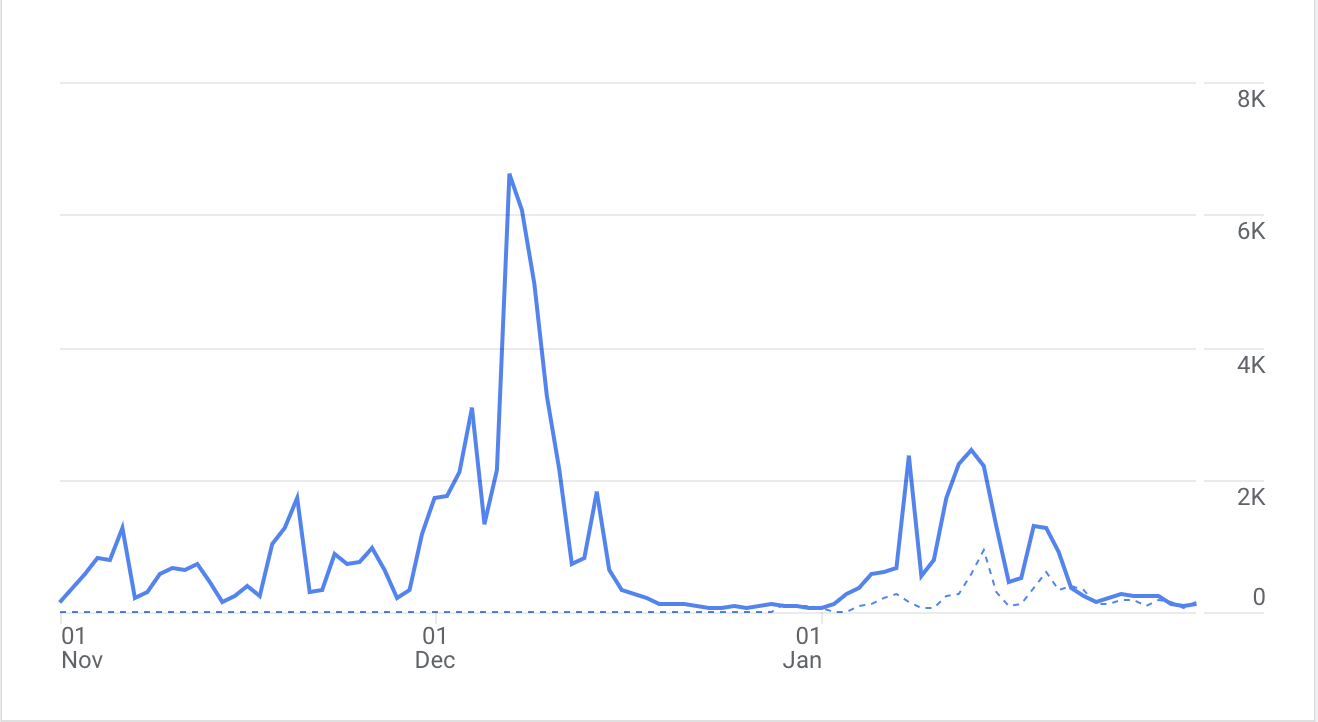
\includegraphics[width=\textwidth]{img/listopad-leden-navstevnost.png}
\caption{Graf návštěvnosti portálu \bso{} od listopadu 2020 do ledna 2021}\label{fig:navstevnost}
\end{figure}

\subsection{Zapojení škol}

Během prvních 14-ti dní projektu se v Pardubickém kraji, díky podpoře odboru školství, zapojilo více jak 60\% středních škol.
V ostatních krajích bylo, i přes podporu \acrshort{msmt}, zapojení škol pouze sporadické.
Pokrok ale nastal po zapojení Úřadu práce na celostátní úrovni,
kdy jediný dopis informačním a poradenským střediskům přinesl zapojení více než 250 škol z celé České Republiky.

\begin{figure}[H]
\centering
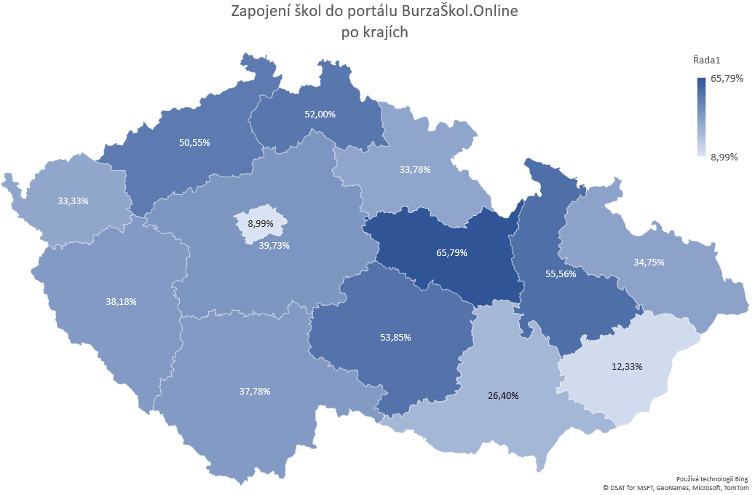
\includegraphics[width=\textwidth]{img/kraje-zapojeni.png}
\caption{Zapojení škol v jednotlivých krajích}\label{fig:kraje-zapojeni}
\end{figure}

\subsection{Přínos aplikace}

Přínos aplikace jsme rozdělili do hlavních šesti bodů:

\begin{enumerate}
  \item Vymysleli jsme nový kanál pro komunikaci mezi uchazeči a středními školami, který v době pandemie alespoň částečně nahradil klasické prezenční výstavy středních škol.
    Využili jsme možností on-line konferencí, které jsme podpořili internetovým portálem pro vyhledávání škol podle vhodných kategorií (geografická lokace, zaměření, obory, úroveň vzdělání, \ldots).

  \item Agregovali jsme dosud nevyžité a opomíjené veřejné zdroje dat o školách (výsledky státních maturit, výsledky soutěží pořádaných \acrshort{msmt}, zprávy České školní inspekce)
    do  jednoho portálu a umožnili jsme porovnávání škol.

  \item Dokázali jsme celý portál \uv{oživit}. Aktivně se do něj zapojilo 465 středních škol a učilišť z celé ČR (více než \(\frac{1}{3}\)).
    Informovali jsme o něm všechny základní školy v ČR.

  \item \uv{Navedli} jsme střední školy v ČR, aby zorganizovaly své dny otevřených dveří pomocí on-line konferencí.
  \item Ve školním roce 2020/21 pomohl náš portál s volbou školy přibližně v 15 tisících případů. 
    Přes portál proběhlo přes 43 tisíc pokusů o on-line propojení mezi návštěvníky a školou.
    Podle zkušenosti z naší školy byl poměr mezi těmito pokusy a skutečnými smysluplnými připojeními přibližně 3:1. 

  \item Zajistili jsme zachování našich přínosů i do budoucna. Funkcionalitu portálu v současné době zapojujeme do předního českého portálu pro vyhledávání škol s historií od roku 2012.
  %\item Vytvořili jsme prostor pro naše mladší spolužáky, aby mohli zlepšovat své programátorské dovednosti na nějakém reálném projektu.
  %\item Pomohli jsme vylepšit rozpočet naší školy o cca 750 tisíc Kč.
\end{enumerate}

% tohle musí přesvědčit porotu o společenském přínosu, smysluplnosti aplikace 

% kolik v systému bylo škol, kdy byl nasazen poprvé a kolik se přes něj uskutečnilo spojení.
